%\documentclass[handout]{beamer}
\documentclass[•]{beamer}
\usepackage[latin1]{inputenc}
\usepackage{amsmath}
\usetheme{Luebeck}
\setbeamertemplate{footline}[frame number] 
\setbeamertemplate{navigation symbols}{} 

\newtheorem{proposition}{Proposition}
\newtheorem{exercise}{Exercise}
\theoremstyle{remark}
\newtheorem{remark}[theorem]{Remark}

\mathchardef\sa="303A
\newcommand{\esup}{\mathop{{\rm ess\,sup}}\limits}
\let\Eqnarray=\eqnarray
\renewcommand{\eqnarray}{\arraycolsep=0.1675em \Eqnarray}

\newcommand{\lag}{\mathcal{L}}
\newcommand{\e}{\mathrm{e}}

% enumabc
%
\makeatletter
\newcommand{\enumabc}
	{\expandafter\def\csname the\@enumctr \endcsname{\alph{\@enumctr}}%
	 \expandafter\def\csname label\@enumctr \endcsname
		{\rm(\csname the\@enumctr \endcsname)}}%
\newcommand{\enuminc}[1]{\addtocounter{\@enumctr}{#1}}
\makeatother
%
\title{Covering the sphere with noncontextuality
inequalities}
\subtitle{Bachelor's thesis in mathematics}
\author{Patrik Hallsj\"{o} \\ Supervisor: Jan-\AA ke Larsson}
\date{}

\AtBeginSection[]
{
  \begin{frame}
    \frametitle{Table of Contents}
    \tableofcontents[currentsection]
  \end{frame}
}
\AtBeginSubsection[]
{
  \begin{frame}
    \frametitle{Table of Contents}
    \tableofcontents[currentsection,currentsubsection]
  \end{frame}
}

\begin{document}
\begin{frame}
\titlepage
\end{frame}
%\begin{frame}
%\tableofcontents
%\end{frame}
\section{Introduction}
\begin{frame}[shrink=10]\frametitle{Introduction}
\begin{block}

In this Bachelor's thesis the following question was answered:\\
Does the inequality posed in the article Klyachko et al [2008] cover the real
part of the Bloch surface of a 3D quantum system when used as in Kochen
and Specker [1967]?
\end{block}
\pause
\begin{remark}
However to understand the questions, some introduction is needed.
\end{remark}
\end{frame}
\subsection{Quantum mechanics}
\begin{frame}[shrink=10]\frametitle{A brief introduction}
\begin{block}

In the beginning of the 20th century, some physical phenomena could not be
explained by classical physics.
\pause


It was these phenomena that led to the formulation of
quantum mechanics. \\
\pause
The basis equation in quantum mechanics is known as Schr\"odingers equation:
\begin{equation*} 
i\hbar\frac{\partial}{\partial t}\psi (\vec{x}, t) = \hat{H}\psi (\vec{x}, t)
\end{equation*}
which is a vector equation and requires the Hamiltonian for a system.
\end{block}
\end{frame}
\begin{frame}[shrink=10]\frametitle{Notation}
\begin{block}

From here on the vector, also known as wave-function will be denoted as a state: $|\psi\rangle$.
Here also the dependent variables are omitted for simplicity such that: 
$$|\psi\rangle = \psi (\vec{x}, t)$$ 
\end{block}
\pause
\begin{example}
Using the notation above, systems with a single particle and spin 1/2 can be written
$$ \psi\rangle =a_0|+\frac{1}{2}\rangle+a_1|-\frac{1}{2}\rangle$$
\end{example}
\end{frame}
\begin{frame}
\begin{example}
However, in the thesis mostly spin 1 is considered, which can be written in the following way:
$$|\psi\rangle=a_0|-1\rangle+a_1|0\rangle+a_2|1\rangle$$
\end{example}
\end{frame}
\begin{frame}\frametitle{Bloch sphere}
\begin{block}

The Bloch sphere is a simple way to represent all possible quantum states. Originally used only for spin 1/2, it can be used for spin 1 systems by  the restriction in our question, to only include the real part of spin 1 systems. 
\end{block}
\end{frame}
\begin{frame}

\begin{figure}[h]
\begin{center}
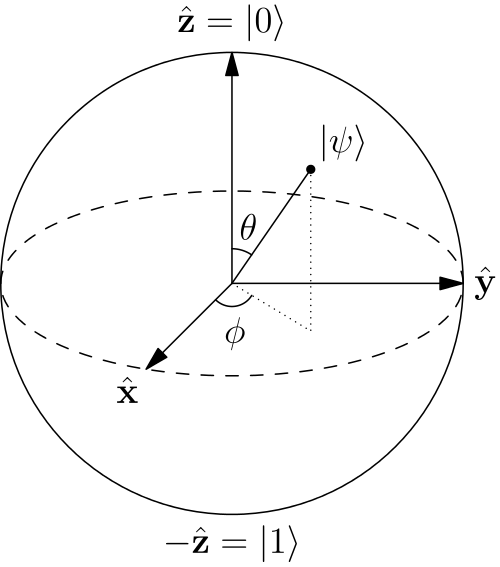
\includegraphics[scale=0.3]{Bloch_Sphere.png} 
\caption{A figure of the Bloch sphere for a spin 1/2 system.}
\end{center}
\end{figure}
\end{frame}



\subsection{Non-contextuality inequalities}
\begin{frame}[shrink=10]\frametitle{Contextuality}
\begin{block}

\begin{itemize}
\item Contextuality refers to when the result of an experiment depends on the context
of the experiment. \pause
\item The opposite of this is of course non-contextuality where the commuting property is not dependent on the experiment. \pause
\item The noncontextuality inequalities are found through the hidden variable
schema which means that they might not hold for a quantum mechanical schema. \pause
\item The interesting case is where the inequality is violated in a quantum mechanical
description.
\end{itemize}
\end{block}
\end{frame}
\begin{frame}[shrink=10]\frametitle{The inequality}
\begin{block}

Klyachko inequality.
\begin{equation*} \label{eq:Inequality}
\langle A_1 A_2 \rangle + \langle A_2 A_3 \rangle + \langle A_3 A_4 \rangle + \langle A_4 A_5 \rangle +
\langle A_5 A_1 \rangle \geq -3
\end{equation*}
This inequality, known as the pentagram inequality, is if violated for a state proves that the state has a nonclassical behaviour. The pentagram inequality is valid for only non-contextual hidden variables.
\end{block}
\end{frame}

\begin{frame}\frametitle{Kochen
and Specker}
\begin{block}

\begin{itemize}
\item Another interesting theorem used for quantum-mechanical contextuality is the
Kochen-Specker theorem. \pause

\item The theorem proves that quantum-mechanics can not be described by a hidden variable schema,thus observables always have definite values and that the observables are non-contextual. \pause

\item Get 117 vectors.
\end{itemize}
\end{block}
\end{frame}

\section{Methods}
\begin{frame}[shrink=10]\frametitle{The vectors}
\begin{block}

Using the vectors given from Kochen
and Specker [1967]. These are used to evaluate the inequality, producing quadratic forms that are then drawn upon the Bloch sphere.
Using the following vectors: \pause
\begin{equation*}
|\psi_1>=
\begin{pmatrix}
0.0000\\
0.0000\\
1.0000\\
\end{pmatrix}
,
|\psi_2>=
\begin{pmatrix}
0.5904\\
0.8071\\
0.0000\\
\end{pmatrix}
,
|\psi_3>=
\begin{pmatrix}
-0.7071\\
0.5172\\
0.4822\\
\end{pmatrix}
,
\end{equation*}
\begin{equation*}
|\psi_4>=
\begin{pmatrix}
0.7071\\
0.5172\\
0.4822\\
\end{pmatrix}
,
|\psi_5>=
\begin{pmatrix}
-0.5904\\
0.8071\\
0.0000\\
\end{pmatrix}
\end{equation*}
will produce the following image,
\end{block}
\end{frame}
\begin{frame}
\begin{figure}[h!]
\begin{center}
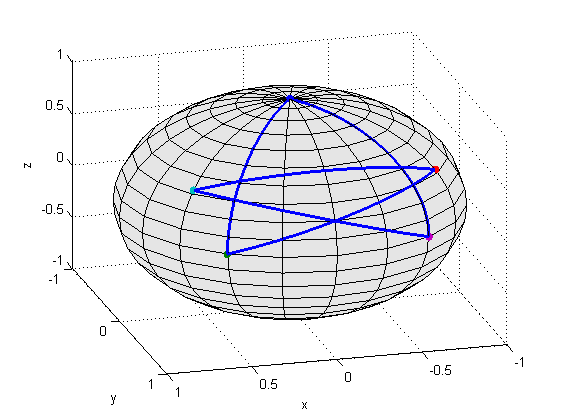
\includegraphics[scale=0.6]{penta1.png}
\caption{The vectors plotted on the sphere.}
\end{center}
\end{figure}
\end{frame}

\begin{frame}[shrink=10]\frametitle{The inequality}
\begin{block}

Klyachko inequality.
\begin{equation*} 
\langle A_1 A_2 \rangle + \langle A_2 A_3 \rangle + \langle A_3 A_4 \rangle + \langle A_4 A_5 \rangle +
\langle A_5 A_1 \rangle \geq -3
\end{equation*}
This inequality, known as the pentagram inequality, is if violated for a state proves that the state has a nonclassical behaviour. The pentagram inequality is valid for only non-contextual hidden variables.
\end{block}
\end{frame}

\begin{frame}[shrink=20]\frametitle{Continuing covering the sphere}

\begin{figure}[h!]
\begin{center}
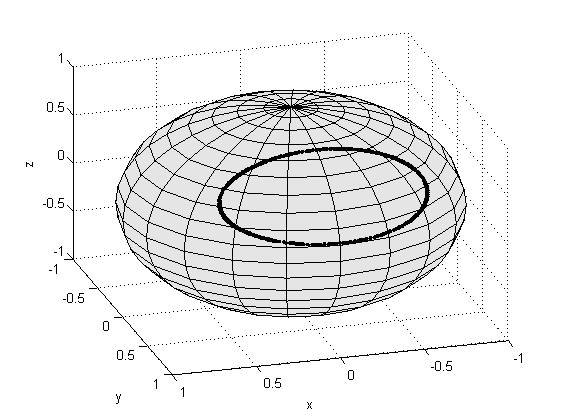
\includegraphics[scale=0.6]{ine1.png}
\caption{The Klyachko inequality plotted on the sphere.}
\end{center}
\end{figure}
\end{frame}
\begin{frame}[shrink=10]
\begin{block}

More vectors and inequalities can be created by rotating the first vectors around the x-axis and the (1,1,1)-axis.
\end{block}
\end{frame}
\section{Data and results}
\begin{frame}[shrink=10]\frametitle{Producing bands}
\begin{figure}[h!]
\begin{center}
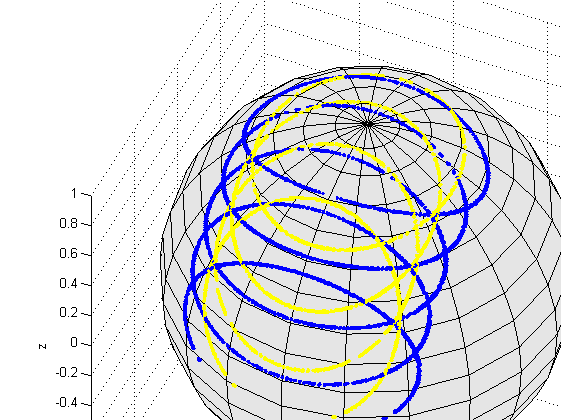
\includegraphics[scale=0.4]{ine12all.png}
\caption{By rotating the vectors around the x-axis and getting new inequalities a band will be created.}
\end{center}
\end{figure}
\end{frame}

\begin{frame}
\begin{figure}[h!]
\begin{center}
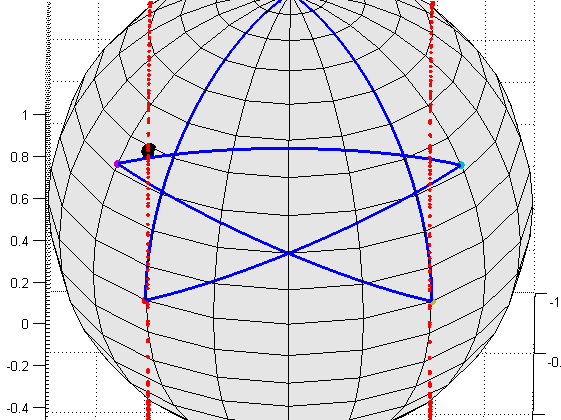
\includegraphics[scale=0.4]{completeband111big.png}
\caption{By rotating the vectors around the x-axis and getting new inequalities a band will be created.}
\end{center}
\end{figure}
\end{frame}
\begin{frame}
\begin{figure}[h!]
\begin{center}
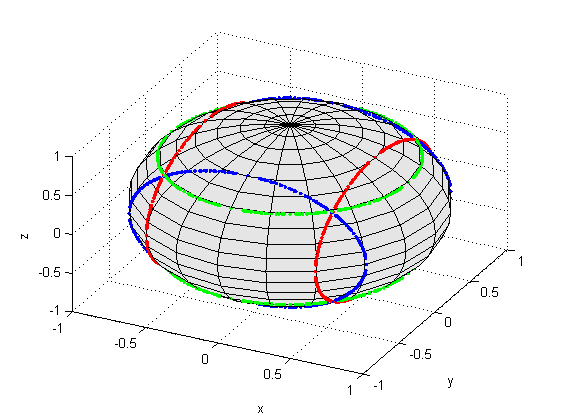
\includegraphics[scale=0.5]{coveredsphere.png}
\caption{Rotating the band around the (1,1,1)-axis will produce the following final result.}
\end{center}
\end{figure}
\end{frame}
\section{Conclusions}
\begin{frame}[shrink=10]\frametitle{Was the question answered?}
\begin{block}

\begin{itemize}
\item It seems that the whole sphere is covered by these inequalities, what does this mean?\\ 
\pause
\item If the whole Bloch sphere is either inside or on the border of the inequalities as seen in the, this means that all possible states of a spin 1 system can be explained by quantum mechanics.
\\
\pause
\item Remember though that there were a few restrictions given.
\\
\pause
\item It is quite undeniable that a proof that the inequality covers all of the real states has been found, however nothing has been said about those which require a complex representation. 
\end{itemize}
\end{block}
\end{frame}
\begin{frame}[shrink=10]\frametitle{Further research to be done}
\begin{block}

\begin{itemize}
\item Complex coefficients.\\
Would fully answer the question. Not that hard, though would loose the visualization which was prioritized.
\pause
\item Other spin systems\\
Mostly spin $\frac{1}{2}$ systems are of interest and in this thesis spin 1 systems were discussed.
There are more spin systems.

\end{itemize}

\end{block}
\end{frame}



\end{document}